\section{The operational model}

The simulacrum used for all agents in the following chapters shall be the
three-dimensional model of the unicycle; its motion shall be expressed by the
nonlinear continuous-time kinematic equations

\begin{align}
  \dot{x}       &= v \cos\theta \\
  \dot{y}       &= v \sin\theta \\
  \dot{\theta}  &= \omega
\label{eq:unicycle_kinematic}
\end{align}

with $\vect{z} = [x,y,\theta]^{\top}$ the vector of states,
$\vect{u} = [v, \omega]^{\top}$ the vector of inputs, and $\dot{\vect{z}} =
f(\vect{z}, \vect{u})$ the (model) system's equation. We consider that
$\vect{x} \in X$, $\vect{y} \in Y$ where $X \equiv Y \equiv \mathbb{R}$,
$\theta \in \Theta \equiv (-\pi, \pi]$ and $\vect{u} \in \mathcal{U}$.
In this 2D spatial environment, the obstacles of the workspace along with the
workspace boundary itself assume an appropriately reformed form: that of a
circle. The labeled space in which an arbitrary agent $i$ moves, along with the
spherical-obstacles-transformed to circles, is depicted in figure
\eqref{fig:unicycle_figure}.

\begin{figure}[H]\centering
  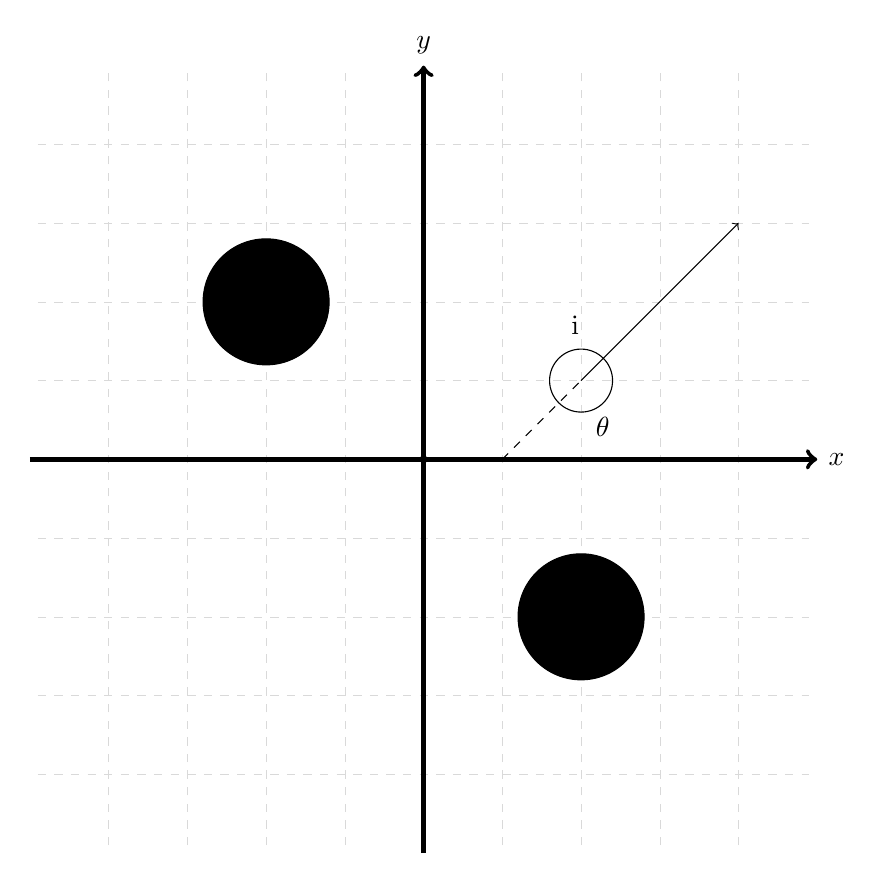
\begin{tikzpicture}
\draw[help lines, color=gray!30, dashed] (-4.9,-4.9) grid (4.9,4.9);
\coordinate (origo) at (0,0);
\coordinate (origo1) at (1.45,0);
\fill[black] (origo) circle (0.05);
\draw[->,ultra thick] (-5,0)--(5,0) node (x) [right]{$x$};
\draw[->,ultra thick] (0,-5)--(0,5) node (y) [above]{$y$};
\draw[] (2.1,1.7) node (i) [left]{i};
\draw[dashed] (1,0)--(2,1);
\draw[->] (2,1)--(4,3);
\draw (x) +(172:3) node {$\theta$};
\tkzDrawArc[R with nodes,](origo1,0.4)(x,y)


\draw[fill] (-2,2) circle [radius=0.8];
\draw[fill] (2,-2) circle [radius=0.8];
\draw (2,1) circle [radius=0.4];
\end{tikzpicture}

  \caption{The 2D plane, agent $i$, whose orientation relative to the $x$
    axis is $\theta$, and two obstacles.}
  \label{fig:unicycle_figure}
\end{figure}

The desired configuration shall be denoted by $\vect{z}_{des}$,
the error dynamics by $\dot{\vect{e}} = g(\vect{e}, \vect{u})$
where $\vect{e}(t) = \vect{z}(t) - \vect{z}_{des}$ and
$\vect{e} \in \mathcal{E} \equiv X \times Y \times \Theta \ominus \vect{z}_{des}$.

\begin{lemma}
  \label{lemma:lipschitz_unicycle}
  Function $g$ is Lipschitz continuous in $\mathcal{E} \times \mathcal{U}$ with
  a Lipschitz constant $$L_g = v \sqrt{Q_{1,1}+Q_{1,2}+Q_{2,1}+Q_{2,2}}$$
  where $\mat{Q} = Q_{\mu\nu}$ is the $3 \times 3$ matrix used to weigh the
  norms involved.
\end{lemma}
